\documentclass[xcolor=table]{beamer}
%\usepackage[utf8]{inputenc}
%\usetheme{Warsaw}
\usetheme{CambridgeUS}
%\usecolortheme{seahorse}

%-------------------------------------------------------------------------------
%          -Packages nécessaires pour écrire en Français et en UTF8-
%-------------------------------------------------------------------------------
\usepackage[utf8]{inputenc}
\usepackage[frenchb]{babel}
\usepackage[T1]{fontenc}
\usepackage{lmodern}
\usepackage{textcomp}

%-------------------------------------------------------------------------------

%-------------------------------------------------------------------------------
%                          -Outils de mise en forme-
%-------------------------------------------------------------------------------
\usepackage{hyperref}
\hypersetup{pdfstartview=XYZ}
\usepackage{enumerate}
\usepackage{graphicx}
%\usepackage{multicol}
%\usepackage{tabularx}

%\usepackage{anysize} %%pour pouvoir mettre les marges qu'on veut
%\marginsize{2.5cm}{2.5cm}{2.5cm}{2.5cm}

\usepackage{indentfirst} %%pour que les premier paragraphes soient aussi indentés
\usepackage{verbatim}
%\usepackage[table]{xcolor}  
%\usepackage{multirow}
\usepackage{ulem}
%-------------------------------------------------------------------------------


%-------------------------------------------------------------------------------
%                  -Nécessaires pour écrire des mathématiques-
%-------------------------------------------------------------------------------
\usepackage{amsfonts}
\usepackage{amssymb}
\usepackage{amsmath}
\usepackage{amsthm}
\usepackage{tikz}
\usepackage{xlop}
\usepackage[output-decimal-marker={,}]{siunitx}
%-------------------------------------------------------------------------------


%-------------------------------------------------------------------------------
%                    - Mise en forme 
%-------------------------------------------------------------------------------

\newcommand{\bu}[1]{\underline{\textbf{#1}}}


\usepackage{ifthen}


\newcommand{\ifTrue}[2]{\ifthenelse{\equal{#1}{true}}{#2}{$\qquad \qquad$}}

\newcommand{\kword}[1]{\textcolor{red}{\underline{#1}}}


%-------------------------------------------------------------------------------



%-------------------------------------------------------------------------------
%                    - Racourcis d'écriture -
%-------------------------------------------------------------------------------

% Angles orientés (couples de vecteurs)
\newcommand{\aopp}[2]{(\vec{#1}, \vec{#2})} %Les deuc vecteurs sont positifs
\newcommand{\aopn}[2]{(\vec{#1}, -\vec{#2})} %Le second vecteur est négatif
\newcommand{\aonp}[2]{(-\vec{#1}, \vec{#2})} %Le premier vecteur est négatif
\newcommand{\aonn}[2]{(-\vec{#1}, -\vec{#2})} %Les deux vecteurs sont négatifs

%Ensembles mathématiques
\newcommand{\naturels}{\mathbb{N}} %Nombres naturels
\newcommand{\relatifs}{\mathbb{Z}} %Nombres relatifs
\newcommand{\rationnels}{\mathbb{Q}} %Nombres rationnels
\newcommand{\reels}{\mathbb{R}} %Nombres réels
\newcommand{\complexes}{\mathbb{C}} %Nombres complexes


%Intégration des parenthèses aux cosinus
\newcommand{\cosP}[1]{\cos\left(#1\right)}
\newcommand{\sinP}[1]{\sin\left(#1\right)}

%Fractions
\newcommand{\myfrac}[2]{{\LARGE $\frac{#1}{#2}$}}

%Vocabulaire courrant
\newcommand{\cad}{c'est-à-dire}

%Droites
\newcommand{\dte}[1]{droite $(#1)$}
\newcommand{\fig}[1]{figure $#1$}
\newcommand{\sym}{symétrique}
\newcommand{\syms}{symétriques}
\newcommand{\asym}{axe de symétrie}
\newcommand{\asyms}{axes de symétrie}
\newcommand{\seg}[1]{$[#1]$}
\newcommand{\monAngle}[1]{$\widehat{#1}$}
\newcommand{\bissec}{bissectrice}
\newcommand{\mediat}{médiatrice}
\newcommand{\ddte}[1]{$[#1)$}

%Figures
\newcommand{\para}{parallélogramme}
\newcommand{\paras}{parallélogrammes}
\newcommand{\myquad}{quadrilatère}
\newcommand{\myquads}{quadrilatères}
\newcommand{\co}{côtés opposés}
\newcommand{\diag}{diagonale}
\newcommand{\diags}{diagonales}
\newcommand{\supp}{supplémentaires}
\newcommand{\car}{carré}
\newcommand{\cars}{carrés}
\newcommand{\rect}{rectangle}
\newcommand{\rects}{rectangles}
\newcommand{\los}{losange}
\newcommand{\loss}{losanges}


%----------------------------------------------------

\title{Périmètres et aires}
\author{}\institute{}


\AtBeginSubsection[]
{
	\begin{frame}
		\frametitle{}
		\tableofcontents[currentsection, currentsubsection]
	\end{frame} 
}

\begin{document}
	
	
	
\begin{frame}
	\titlepage
\end{frame}

\section{Périmètre}

\subsection{Définition}

\begin{frame}
\frametitle{ }  
\framesubtitle{ }	

\begin{exampleblock}{Définition}
	Le \bu{périmètre} d'une figure est la \underline{longueur du contour} de cette figure.
\end{exampleblock}

\begin{block}{Exemple}
	\begin{columns}[onlytextwidth]
		\begin{column}{0.465\textwidth}
			\center{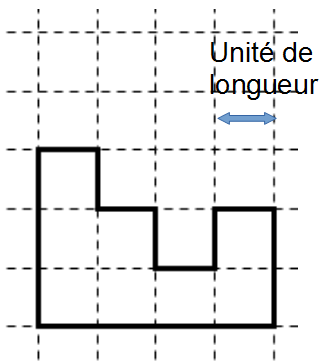
\includegraphics[scale=0.55]{./img/aire}}			
		\end{column}
		\begin{column}{0.465\textwidth}
			Le périmètre de cette figure est 16 unités de longueur.			
		\end{column}
	\end{columns}
		
\end{block}	


\end{frame}

\subsection{Unité de longueur}
\begin{frame}
	\frametitle{}  
	\framesubtitle{}	
	
	\begin{exampleblock}{Définition}
		La mesure d'une \bu{longueur} dépend de l'unité choisie.
		L'unité légale de longueur est le \bu{metre} (m).		
	\end{exampleblock}
	
	\begin{alertblock}{Autres unités de longueur}
		\tiny{\begin{tabular}{|c|c|c|c|c|c|c|}
	\hline
		\rowcolor{gray} \multicolumn{3}{|c|}{\textbf{\underline{Multiples} de l'unité}} & \textbf{Unité} & \multicolumn{3}{c|}{\textbf{\underline{Sous-multiples} de l'unité}} \\
	\hline
		\textbf{Kilo}mètre & \textbf{hecto}mètre & \textbf{déca}mètre & \bu{mètre} & \textbf{déci}mètre & \textbf{centi}mètre & \textbf{milli}mètre \\
	\hline
		1 km $=$ 1 000 m & 1hm $=$ 100 m & 1 dam $=$ 10 m & 1m & 1 dm $=$ 0,1 m & 1 cm $=$ 0,01 m & 1 mm $=$ 0,001 m \\
	\hline
	
\end{tabular}}
	\end{alertblock}
		
\end{frame}

\begin{frame}
	\frametitle{}  
	\framesubtitle{}	
	
	\begin{alertblock}{Autres unités de longueur}
		\tiny{\begin{tabular}{|c|c|c|c|c|c|c|}
	\hline
		\rowcolor{gray} \multicolumn{3}{|c|}{\textbf{\underline{Multiples} de l'unité}} & \textbf{Unité} & \multicolumn{3}{c|}{\textbf{\underline{Sous-multiples} de l'unité}} \\
	\hline
		\textbf{Kilo}mètre & \textbf{hecto}mètre & \textbf{déca}mètre & \bu{mètre} & \textbf{déci}mètre & \textbf{centi}mètre & \textbf{milli}mètre \\
	\hline
		1 km $=$ 1 000 m & 1hm $=$ 100 m & 1 dam $=$ 10 m & 1m & 1 dm $=$ 0,1 m & 1 cm $=$ 0,01 m & 1 mm $=$ 0,001 m \\
	\hline
	
\end{tabular}}
	\end{alertblock}
	
	\begin{columns}[onlytextwidth]
		\begin{column}{0.64\textwidth}
			\begin{block}{Exemple}
				On veut calculer le périmètre de la figure ci-contre : 
				
				\begin{small}
					\begin{itemize}
						\item 32 mm $=$ 3,2 cm et 0,31~dm~$=$~3,1~cm
						\item[P=]  AB + BC + CD + DE + EA
						\item[P=] 2 + 3,2 + 2,2 + 3 + 3,1 
						\item[P=] 13,5
						\item[$\rightarrow$] Le périmètre du polygone ABCDE est 13,5 cm.
					\end{itemize}	
				\end{small}
				
				 
				
				
			\end{block}
		\end{column}
		\begin{column}{0.35\textwidth}
			\center{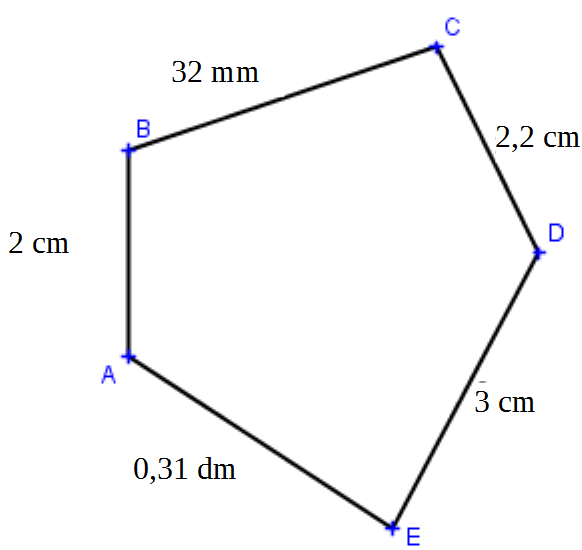
\includegraphics[scale=0.32]{./img/figure}}			
		\end{column}
	\end{columns}
	
\end{frame}

\begin{frame}
	\frametitle{Convertir les unités de longueur}  
	\framesubtitle{À l'aide du tableau de conversion}	
	
	On utilise le tableau ci-dessous :
		\begin{small}
		\begin{center}
			\begin{tabular}{|c|c|c|c|c|c|c|}	
				\hline
					\rowcolor{gray} ~~\textbf{km}~~    &    ~~\textbf{hm}~~ &    ~~\textbf{dam}~~ & ~~\textbf{m}~~ & ~~\textbf{dm}~~ & 	~~\textbf{cm}~~ & ~~\textbf{mm}~~ \\
				\hline
					& & & & & & \\
				\hline	
			\end{tabular}	\pause
		\end{center}
		\end{small}

	
	\begin{block}{Exemple}
		On veut convertir 7,548 hm en m.
		\begin{itemize}
			\item[$\rightarrow$] On met un chiffre par case dans le tableau, en commençant par les unités du nombre de départ. Puis on place la virgule à la nouvelle unité choisie (en ajoutant des zéro si nécessaire)
		\end{itemize}
		
		\begin{small}		
		\begin{center}
			\begin{tabular}{|c|c|c|c|c|c|c|}	
				\hline
				\rowcolor{gray} ~~\textbf{km}~~    &    ~~\textbf{hm}~~ &    ~~\textbf{dam}~~ & ~~\textbf{m}~~ & ~~\textbf{dm}~~ & 	~~\textbf{cm}~~ & ~~\textbf{mm}~~ \\
				\hline
					& 7 & 5 & 4, & 8 & & \\
				\hline	
			\end{tabular}	
		\end{center}
		\end{small}
		
		CONCLUSION : 7,548 hm = 754,8 m.
	\end{block}
	
	
\end{frame}

\begin{frame}
	\frametitle{Convertir les unités de longueur}  
	\framesubtitle{En multipliant ou en divisant directement par 10; 100; 1000 ...}	
	
	\begin{alertblock}{Méthode}
		On peut convertir directement les unités de longueur à l'aide de multiplications et de divisions par 10; 100; 1000 ...
	\end{alertblock}\pause
	
	\begin{block}{Exemple}
		\begin{itemize}
			\item On veut convertir 32,45 m en cm.
			\item On sait que 1 m $=$ 100 cm.
			\item[$\rightarrow$] 32,45 $\times$ \textbf{100} $=$ 3 245.
		\end{itemize}
		
		Donc 32,45 m $=$ 3 245 cm.		
	\end{block}
	
\end{frame}

\section{Formules de calcul du périmètre}

\subsection{Triangles}

\begin{frame}
	\frametitle{}  
	\framesubtitle{}	
	
	%\begin{alertblock}{Règle générale}
		Le périmètre d'un triangle est égal à la \underline{somme des longueurs de ses} \underline{ trois côtés}.
	%\end{alertblock}
	
	

	\begin{columns}[onlytextwidth]
		\begin{column}{0.48\textwidth}
			\begin{alertblock}{Triangle isocèle}<2->
				\center{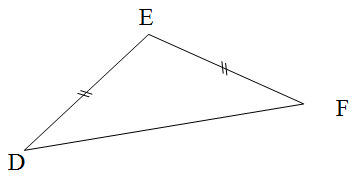
\includegraphics[scale=0.45]{./img/iso}}
				\begin{itemize}
					\item Périmètre = 2 x longueur des côtés égaux + longueur de la base
					\item $P = 2 \times\ EF + DF$
				\end{itemize}
				
			\end{alertblock}
		\end{column}
		\begin{column}{0.48\textwidth}
			\begin{alertblock}{Triangle équilatéral}<3->
				\center{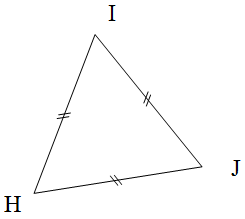
\includegraphics[scale=0.45]{./img/equi}}
				\begin{itemize}
					\item Périmètre = 3 x longueur d'un côté
					\item $P = 3 \times\ IJ $
				\end{itemize}
				
			\end{alertblock}
		\end{column}
	\end{columns}
	
	
\end{frame}

\subsection{Quadrilatères}

\begin{frame}
	\frametitle{}  
	\framesubtitle{}	
	
	%\begin{alertblock}{Règle générale}
	Le périmètre d'un quadrilatère est égal à la \underline{somme des longueurs de ses} \underline{quatre côtés}.
	%\end{alertblock}
	
	
	
	\begin{columns}[onlytextwidth]
		\begin{column}{0.3\textwidth}
			\begin{alertblock}{Losange}<2->
				\center{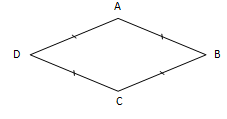
\includegraphics[scale=0.45]{./img/los}}
				\begin{itemize}
					\item Périmètre = 4 x longueur d'un côté
					\item $P = 4 \times\ c$
					\item $P = 4 \times\ AB$
				\end{itemize}
				
			\end{alertblock}
		\end{column}
		\begin{column}{0.35\textwidth}
			\begin{alertblock}{Rectangle}<3->
				\center{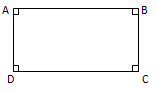
\includegraphics[scale=0.45]{./img/rect}}
				\begin{itemize}
					\item Périmètre = 2 $\times$ (longueur $+$ largeur) ou
					\item Périmètre = 2 $\times$ longueur $+$  2 $\times$ largeur)
					\item $P = 2 \times L + 2 \times l$
					\item $P = 2 \times AB + 2 \times BC$
				\end{itemize}
				
			\end{alertblock}
		\end{column}
		\begin{column}{0.25\textwidth}
			\begin{alertblock}{Carré}<4->
				\center{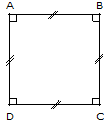
\includegraphics[scale=0.45]{./img/carre}}
				\begin{itemize}
					\item Périmètre = 4 x longueur d'un côté
					\item $P = 4 \times\ c $
					\item $P = 4 \times\ AB $
				\end{itemize}
				
			\end{alertblock}
		\end{column}
	\end{columns}
\end{frame}

\subsection{Cercles}	

\begin{frame}
	\frametitle{}  
	\framesubtitle{}	
	
	\begin{columns}[onlytextwidth]
		\begin{column}{0.3\textwidth}
			\center{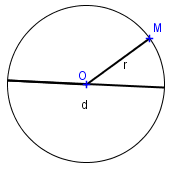
\includegraphics[scale=0.5]{./img/cercle1}}
			
		\end{column}
		\begin{column}{0.7\textwidth}
			La longueur d'un cercle est lié à son rayon (et de son diamètre).
			La longueur d'un cercle de diamètre $d$ et de rayon $r$, s'obtient avec l'une des deux formules suivantes:
			
			\begin{itemize}
				\item $P = \pi \times d$
				\item $P = 2 \times \pi \times r$
			\end{itemize}
			
			La lettre grecque $\pi$ (pi) désigne un nombre qui n'est pas décimal (On ne le connaît pas exactement).
			On prend généralement 3,14 comme valeur approchée de $\pi$ :
			\begin{itemize}
				\item[$\Rightarrow$] $ \pi \approx 3,14$
			\end{itemize}
		\end{column}
	\end{columns}
	
	\begin{block}{Exemple}
		Si $r = 3 cm$, alors : P = $2 \times \pi \times 3 = \pi \times 6 \approx 18,84$
	\end{block}
\end{frame}
	
\section{Aire}

\subsection{Définition}

\begin{frame}
	\frametitle{ }  
	\framesubtitle{ }	
	
	\begin{exampleblock}{Définition}
		La \bu{surface} d'une figure plane est la partie située à l'intérieur de cette figure. \textbf{L'aire} d'une figure est \underline{la mesure de sa surface}.
	\end{exampleblock}
	
	\begin{block}{Exemple}
		\begin{columns}[onlytextwidth]
			\begin{column}{0.465\textwidth}
				\center{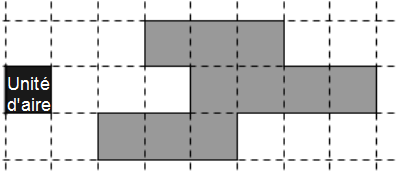
\includegraphics[scale=0.6]{./img/aire1}}			
			\end{column}
			\begin{column}{0.465\textwidth}
				L'aire de cette figure est 10 unités d'aire.			
			\end{column}
		\end{columns}
		
	\end{block}	
	
	
\end{frame}



\begin{frame}
	\frametitle{ }  
	\framesubtitle{ }	
	
	\begin{block}{Remarque}
		\begin{columns}[onlytextwidth]
			\begin{column}{0.465\textwidth}
				Le périmètre et l'aire sont deux grandeurs différentes et indépendantes. Sur la figure ci-contre, le carré gris foncé a une aire plus grande que celle de la figure gris clair, mais son périmètre est plus petit.			
			\end{column}
			\begin{column}{0.465\textwidth}
				\center{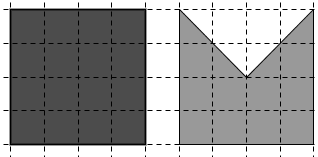
\includegraphics[scale=0.45]{./img/aire2}}			
			\end{column}
			
		\end{columns}
		
	\end{block}	
	
	
\end{frame}

\subsection{Unité d'aire}

\begin{frame}
	\frametitle{}  
	\framesubtitle{}	
	
	\begin{exampleblock}{Définition}
		\begin{itemize}
			\item L'unité légale d'aire est le \bu{metre carré} ($m$²).		
			\item 1$m$² est l'aire d'un carré de 1 m de coté.
		\end{itemize}
		
	\end{exampleblock}
	
	\begin{alertblock}{Autres unités de longueur}
		\scriptsize{\begin{tabular}{|c|c|c|c|c|c|c|}
	\hline
		\rowcolor{gray} \multicolumn{3}{|c|}{\textbf{\underline{Multiples} de l'unité}} & \textbf{Unité} & \multicolumn{3}{c|}{\textbf{\underline{Sous-multiples} de l'unité}} \\
	\hline
		$km^2$ & $hm^2$ & $dam^2$ & $m^2$ & $dm^2$ & $cm^2$ & $mm^2$ \\
	\hline
		 1$km^2$ & 1$hm^2$ & 1 $dam^2$ & & 1$dm^2$ & 1$cm^2$  & 1$mm^2$ \\
		 $=$ & $=$ & $=$ & \textbf{1$m^2$}  & $=$ & $=$  & $=$ \\
 		 $1\:000\:000m^2$ & $10\:000m^2$ & $100m^2$ & & $0,01m^2$ & $0,0001m^2$  & $0,000\:001m^2$ \\
	\hline
	
\end{tabular}}
		\centering{
		\begin{tabular}{ccc}
			\\
			1 $km^2 \:=\:100 hm^2 $ & 1 $hm^2 \:=\:100 dam^2 $ & 1 $dam^2 \:=\:100 m^2 $ \\
			1 $m^2 \:=\:100 dm^2 $ & 1 $dm^2 \:=\:100 cm^2 $ & 1 $cm^2 \:=\:100 mm^2 $
		\end{tabular}}
	\end{alertblock}
	
\end{frame}

\begin{frame}
	\frametitle{Convertir les unités d'aire}  
	\framesubtitle{À l'aide du tableau de conversion}	
	
	On utilise le tableau ci-dessous :
	%\begin{small}
		\begin{center}
			\begin{tabular}{|c|c|c|c|c|c|c|c|c|c|c|c|c|c|}	
				\hline
				\rowcolor{gray} 
				\multicolumn{2}{|c|}{\textbf{$km^2$}}   &    
				\multicolumn{2}{|c|}{\textbf{$hm^2$}} &    \multicolumn{2}{|c|}{\textbf{$dam^2$}} & \multicolumn{2}{|c|}{\textbf{$m^2$}}& \multicolumn{2}{|c|}{\textbf{$dm^2$}} & 	\multicolumn{2}{|c|}{\textbf{$cm^2$}} & \multicolumn{2}{|c|}{\textbf{$mm^2$}} \\
				\hline
				& & & & & & & & & & & & & \\
				\hline	
			\end{tabular}	\pause
		\end{center}
%	\end{small}
	
	
	\begin{block}{Exemple}
		On veut convertir 9,32 $m^2$ en $hm^2$.
		\begin{itemize}
			\item[$\rightarrow$] On met un chiffre par unité dans le tableau, en commençant par les unités du nombre de départ. Puis on place la virgule à la nouvelle unité choisie (en ajoutant des zéro si nécessaire)
		\end{itemize}
		
		%\begin{small}		
			\begin{center}
				\begin{tabular}{|c|c|c|c|c|c|c|c|c|c|c|c|c|c|}	
					\hline
					\rowcolor{gray} 
					\multicolumn{2}{|c|}{\textbf{$km^2$}}   &    
					\multicolumn{2}{|c|}{\textbf{$hm^2$}} &    \multicolumn{2}{|c|}{\textbf{$dam^2$}} & \multicolumn{2}{|c|}{\textbf{$m^2$}}& \multicolumn{2}{|c|}{\textbf{$dm^2$}} & 	\multicolumn{2}{|c|}{\textbf{$cm^2$}} & \multicolumn{2}{|c|}{\textbf{$mm^2$}} \\
					\hline
					& & 
					& 0& 
					0& 0& 
					0& 9& 
					3& 2& 
					& & 
					& \\
					\hline	
				\end{tabular}	\pause
			\end{center}
		%\end{small}
		
		CONCLUSION : 9,32 $m^2$ = 0,000932 $hm^2$.
	\end{block}
	
	
\end{frame}

\section{Formules de calcul du périmètre}

\subsection{Quadrilatères}

\begin{frame}
	\frametitle{}  
	\framesubtitle{}	
	
		
	\begin{columns}[onlytextwidth]
		\begin{column}{0.48\textwidth}
			\begin{alertblock}{Rectangle} %<3->
				\center{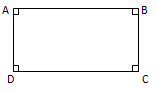
\includegraphics[scale=0.55]{./img/rect}}
				\begin{itemize}
					\item Aire = Longueur $\times$ largeur 
					\item $A = L \times l$
					\item $A = AB \times BC$
				\end{itemize}
				
			\end{alertblock}
		\end{column}
		\begin{column}{0.48\textwidth}
			\begin{alertblock}{Carré} %<4->
				\center{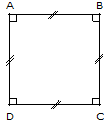
\includegraphics[scale=0.55]{./img/carre}}
				\begin{itemize}
					\item Aire = longueur d'un côté $\times$ longueur d'un côté
					\item $P = c \times\ c $
					\item $P = AB \times\ AB $
				\end{itemize}
				
			\end{alertblock}
		\end{column}
	\end{columns}
\end{frame}

\subsection{Triangles}

\begin{frame}
	\frametitle{}  
	\framesubtitle{}	
	
	
	\begin{columns}[onlytextwidth]
		\begin{column}{0.48\textwidth}
			\begin{alertblock}{Triangle rectangle} %<3->
				\center{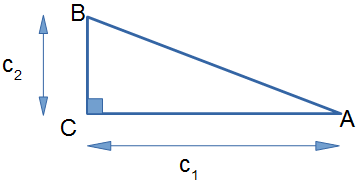
\includegraphics[scale=0.55]{./img/tr}}
				\begin{itemize}
					\item Aire = (coté de l'angle droit $\times$ coté de l'angle droit)$:$2 
					\item $A =$ {\LARGE $\frac{(c_1 \times c_2)}{2}$} 
					\item $A =$ {\LARGE $\frac{(AC \times BC)}{2}$} 
				\end{itemize}
				
			\end{alertblock}
		\end{column}
		\begin{column}{0.48\textwidth}
			\begin{alertblock}{Triangle} %<4->
				\center{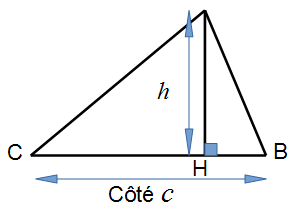
\includegraphics[scale=0.55]{./img/tri}}
				\begin{itemize}
					\item Aire = (côté $\times$ hauteur relative à ce côté)$:$2
					\item $A =$ {\LARGE $\frac{(c \times h)}{2}$} 
					\item $A =$ {\LARGE $\frac{(AH \times BC)}{2}$} 
				\end{itemize}
				
			\end{alertblock}
		\end{column}
	\end{columns}
\end{frame}


\subsection{Disque}	

\begin{frame}
	\frametitle{}  
	\framesubtitle{}	
	
	\begin{columns}[onlytextwidth]
		\begin{column}{0.35\textwidth}
			\center{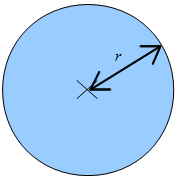
\includegraphics[scale=0.6]{./img/cercle2}}
			
		\end{column}
		\begin{column}{0.65\textwidth}
			L'aire d'un disque de rayon $r$ est égale à \textbf{$A=\pi \times r \times r$}
			
			\begin{block}{Exemple}
				Si $r = 5 cm$, alors : \\
				\begin{tabular}{ccl}
					
					$A $ & $=$ & $\pi \times 5 \times 5$ \\
					$A $ & $=$ & $\pi \times 25$ \\
				\end{tabular}
				
				L'aire de ce disque est exactement $\pi \times 25$ cm².
				
				
				\begin{tabular}{ccl}
					
					$A $ & $\approx$ & $78,5$ \\

				\end{tabular}
				
				L'aire de ce disque est environ égale à $78,5$ cm².
			\end{block}
		\end{column}
	\end{columns}
	
	
\end{frame}

\end{document}




\begin{frame}
	\frametitle{}  
	\framesubtitle{}	
	

\end{frame}